% ------------------------------------------------------------------------------
% A primer on continuum models and how this relates to the work we have done
% 1) Introduce logistic growth and diffusion
% 2) Introduce FKPP in all its glory .
% 3) Show one and two d spread
% 4) Couple to the sub-grid, what this says about the sub-grid...
% 5) Talk about growth rate-xi and growth rate of sub-grid... an assumption about mixing and SIR <--         appendix territory
% 6) Show `toy model properties in xi and d' get realistic looking spread...
% 7) Show realistic spread and give a primer to things which could be done.
% 8) Talk about alternate more, non-linear models and consult Rammile...
% ------------------------------------------------------------------------------

\chapter{Towards landscape-level control}

% In reality, connectivity between patches depend on the dispersal kernel, and not on an arbitrarily defined nearest-neighbour structuring element.
% Connectivity between patches can extend radially non-locally over a number of surrounding patches.

\label{ch7:landscape-level-control}

A great deal of research has been carried out to understand the optimisation of control for plant and and tree-based epidemics\textemdash as reviewed section \ref{chapter2:plant-ecologoy} \textcolor{red}{for a review}. 
Spatial structure is an essential factor when considering how to manage an outbreak \cite{spatial-control-optimisation, control-heterogeneous-landscapes}. 
The main-stream paradigm of control typically considers infected tree removals over a relatively small spatial scale, near infected hosts \cite{WEBIDEMICS}, or more broadly, ahead of the wavefront \cite{large-scale-control}. 
However, landscape-level epidemic control, based solely on the structure of large-scale spatial distribution of hosts incorporating topography, has yet to be explored in-depth.

In this chapter, we will examine how host-heterogeneity, under the influence of a wind-dispersed pathogen, can give rise to natural pinch-points and fault lines in the spatial distribution of hosts. 
Population pinch points may give rise to a bottleneck in the epidemic spread, which in principle, 
may be exploited with targeted tree felling to fragment the host population with minimised effort. 
In essence, a strategy of 'regional containment', targeting the local wind-based pathogen dispersal mechanism, is formulated and scaled up over large spatial scales. Similar concepts for crop and livestock diseases have been outlined \cite{PAPAIX201435, GILIOLI20131, Gilligan-disease-management}, but to our knowledge this has not been generalised to tree populations over large spatial scales.

% - The challenge of controlling ADB reflects the challenge of containing a pathogen that spreads via long-distance dispersal (LDD). 
% Moreover, HP can infect ash through diverse mechanisms such as water-course and contaminated soil and LDD means that new and distant foci can emerge over large distances without the need for nearby ash\textemdash for a more detailed review of ADB, including the challenges of control and biology, see chapter \ref{chapter2:litrevieiw}.
% Subsequently, we found connectedness inside a given cluster could depend on just a small number of `connecting points' which if removed, thinned below $\rho_c$, would lead to significant fragmentation and divide the cluster

% - This leads us to develop a heuristically-based fragmentation algorithm
% - In section X map connectivity will be examined under a threshold function \Phi(\xi). 
% -As we define it, fragmentation considers which locations in the population, if artificially taken below $R_0 = 1$ through felling, would disrupt epidemiological connectivity\textemdash, thus leading to containment. 
% -Epidemic containment in the largest $R_0$-cluster is then analysed and shown to be most applicable over a specific range of infectivity parameters.
% -Although the strategy of control presented in this chapter is demonstrated on a simplified model of ADB, the results are generic and could be applied to any wind-dispersed pathogen.
% - Developing a landscape-level control strategy when there is LDD (and epidemic uncertainty) present several obstacles, 
% - The emergent epidemic caused by the pathosystem ash dieback (ADB) is predicted to wipe out the vast majority of ash in Great Britain over the next few decades \cite{ash-dieback-costs}. 
% - Currently, large-scale control efforts aim to slow the spread, in contrast, to complete containment. % Find references of current efforts/guidelines 
% - A slower rate of spread benefits ash populations allowing them to recover alongside artificial replanting. % reference 

%-----------------------------------
% Suppose two patches of land, having tree densities above the threshold, $R_0 = 1$, are separated by an intermediary patch below the threshold. If we are not careful, dispersal could traverse the below-threshold patch within a single jump, even at local spatial scales. As such, we must choose a domain resolution that gives some assurance that, at the local scale, wind-dispersed spores cannot jump over whole patches with singular jumps. As always, there is the possibility that spores disperse more considerable distances, from mainland Europe to Great Britain, for example, \cite{freer2017tree, wylder2018evidence}. Nevertheless, this chapter aims at targeting dispersal at local scales, and LDD can be omitted for now.
%-----------------------------------

% Classical percolation theory requires lattice points to be independently open or closed, with no dependence on the state of nearest neighbours. So, strictly speaking, the analogy to percolation breaks down because the susceptibility of a given patch of ash is likely dependent on its neighbours $R_0$-value; as can be seen in Figures \ref{fig:uk-mapping}(d-e), particularly in the south of England where ash densities are high. 
% Heterogeneity in the $R_0$-map becomes particularly useful in the the next chapter, where we investigate a potential strategy of landscape-level control based on disrupting epidemic connectivity and fragmentation.
% Before we can move towards epidemic control, it is desirable to understand $R_0$-clustering more fully.
%-----------------------------------
% Assuming connectivity
% Patches below the threshold present a natural barrier to ADB spore dispersal between clusters, for two reasons: 
% 1) Below-threshold patches do not support high levels of infected biomass, spore dispersal emanating from these patches will therefore be lessened.
% 2) The domain resolution, configured in section \ref{ch6:re-scaling-host-data}, ensures that no secondary infections will result for the parameter values and spatial scale under consideration in the seasonal $SEIR$ model of ADB.
% Likewise, 

\section{Method: $R_0$-cluster fragmentation}

In chapter \ref{ch:6-adb}, $R_0$-clusters were introduced.
Cluster detected in the $R_0$-map revealed which regions in Great Britain are likely to be the most severely devastated by the pathogen.
Whereas, patches below the threshold do not support high levels of infected biomass and spore dispersal emanating from these patches are (on average) lessened.
Thus, in this simplified interpretation patches below the threshold present a natural barrier to the spread of disease.
Moving forward, we presume that the pathogen will remain confined within isolated $R_0$-clusters and not spread through patches below $R_0=1$.
Undoubtedly, a number of assumptions underpin this argument including the omission of LDD, both wind-borne and human-mediated, alongside stochastic outbreaks below the threshold\textemdash 
\textcolor{red}{these assumptions are revisited in an `unfinished' case study toward the end of the chapter}.
 
Here, epidemics inside an $R_0$-map are reduced to a `\textit{percolation-like}' problem, with the caveat of clustering. 
If no control is attempted, all patches within a susceptible cluster are put at risk if one patch becomes infected;
this motivates a control strategy based on cluster fragmentation to accomplish regional containment.
Specifically, by artificially reducing $R_0$ in a small number of identified patches, connectivity within the cluster can be efficiently disrupted with minimal effort.
Cluster fragments then define disconnected `sub-clusters' (e.g. $\mathbf{C_1}$ and $\mathbf{C_2}$) that eliminates risk for trees inside one sub-cluster.
Ash trees inside the confining cluster are assumed to be removed by the pathogen while Ash trees inside the remaining sub-cluster survive and remain susceptible.
If the control effort is small in comparison to the reduction of epidemic-impact, then efficient control is achieved.

% - The modelled distribution of ash depicts a continuum of connectivity throughout Great Britain.
% - The shape of each cluster is constrained by landscape topography and geography. 

\subsection{Identifying high-priority patches}

An algorithm was developed to identify high-priority patches in the host distribution, which, if taken below the threshold disrupts epidemic connectivity.
Given a CCA-identified cluster in the $R_0$-map, $\mathbf{C}$, we can define a binary-valued threshold function $\Phi(\xi)$ by:
\begin{align}
\label{eq:xi-step}
\Phi(\xi) = \left\{ \begin{array}{cc} 
                1 & R_0(i, j) \geq \xi \\
                0 & R_0(i, j) < \xi \\
                \end{array} \right.
\end{align}

where $R(i,j)$ is the patch-level reproduction ratio at spatial coordinates $(i,j)$ in $\mathbf{C}$.
The parameter $\xi$ takes values in interval $\big[1, \mathrm{max}\big( R_0(i,j)\big) \big]$, 
where $\mathrm{max}\big(R_0(i, j)\big)$ is the highest value of $R_0$ in $\mathbf{C}$\textemdash henceforth denoted by $R_{max}$.

Figure \ref{fig:R0-threshold-function} shows the how the function $\Phi(\xi)$ allows the identification of high priority spatial locations.
In Figure \ref{fig:R0-threshold-function}(a) we begin with a target-cluster, $\mathbf{C}$, shown in blue;
$\mathbf{C}$ is the largest cluster detected in an arbitrary $R_0$-map for the model $\phi_1$-ga for $\beta^*=450$, as described previously.
Applying the threshold function $\Phi(\xi=1)$ recovers $\mathbf{C}$ entirely, as all patches in $\mathbf{C}$ are over the threshold.
Whereas, larger values of $\xi$ result in a lower-density map with sparsely distributed clusters, 
demonstrated by the small number of labelled clusters in Figure \ref{fig:R0-threshold-function}(b) at $\Phi(\xi=4)$.
Similarly, only one, or at most a handful, of patches populate the domain at the limiting value $\Phi(\xi=R_{max})$.

Connected component analysis (CCA) is performed at each step $\xi \in [1, R_{max}]$ in order to identify and label sub-clusters. 
At particular steps $\xi \rightarrow \xi - \delta\xi$ (i.e. back-stepping), $\mathbf{C}$ will begin to form when distinct sub-clusters\footnote{
It is possible that three or more sub-clusters suddenly connect to form $\mathbf{C}$ in the same step; 
these complexities are taken into account by the algorithm.} 
 (e.g. $\mathbf{C_1}$ and $\mathbf{C_2}$) suddenly connect when certain critical links become non-zero\textemdash
analogous to the formation of a spanning cluster opening up in a percolation. 
Figure \ref{fig:R0-threshold-function}(d) depicts a scenario with a number of disconnected sub-clusters at $\xi=1.19$ that merge together at $\xi=1.15$.
The well-known `binary dilation' operator \cite{liang1989erosion, 23111, nachtegael2001connections} was used to detect all patches that become non-zero and bridge sub-clusters, as elaborated in \textcolor{red}{appendix X}.
Henceforth, patches that connect sub-clusters in a discontinuity-step are refereed to as `connecting patches'.

\begin{figure}
    \centering
    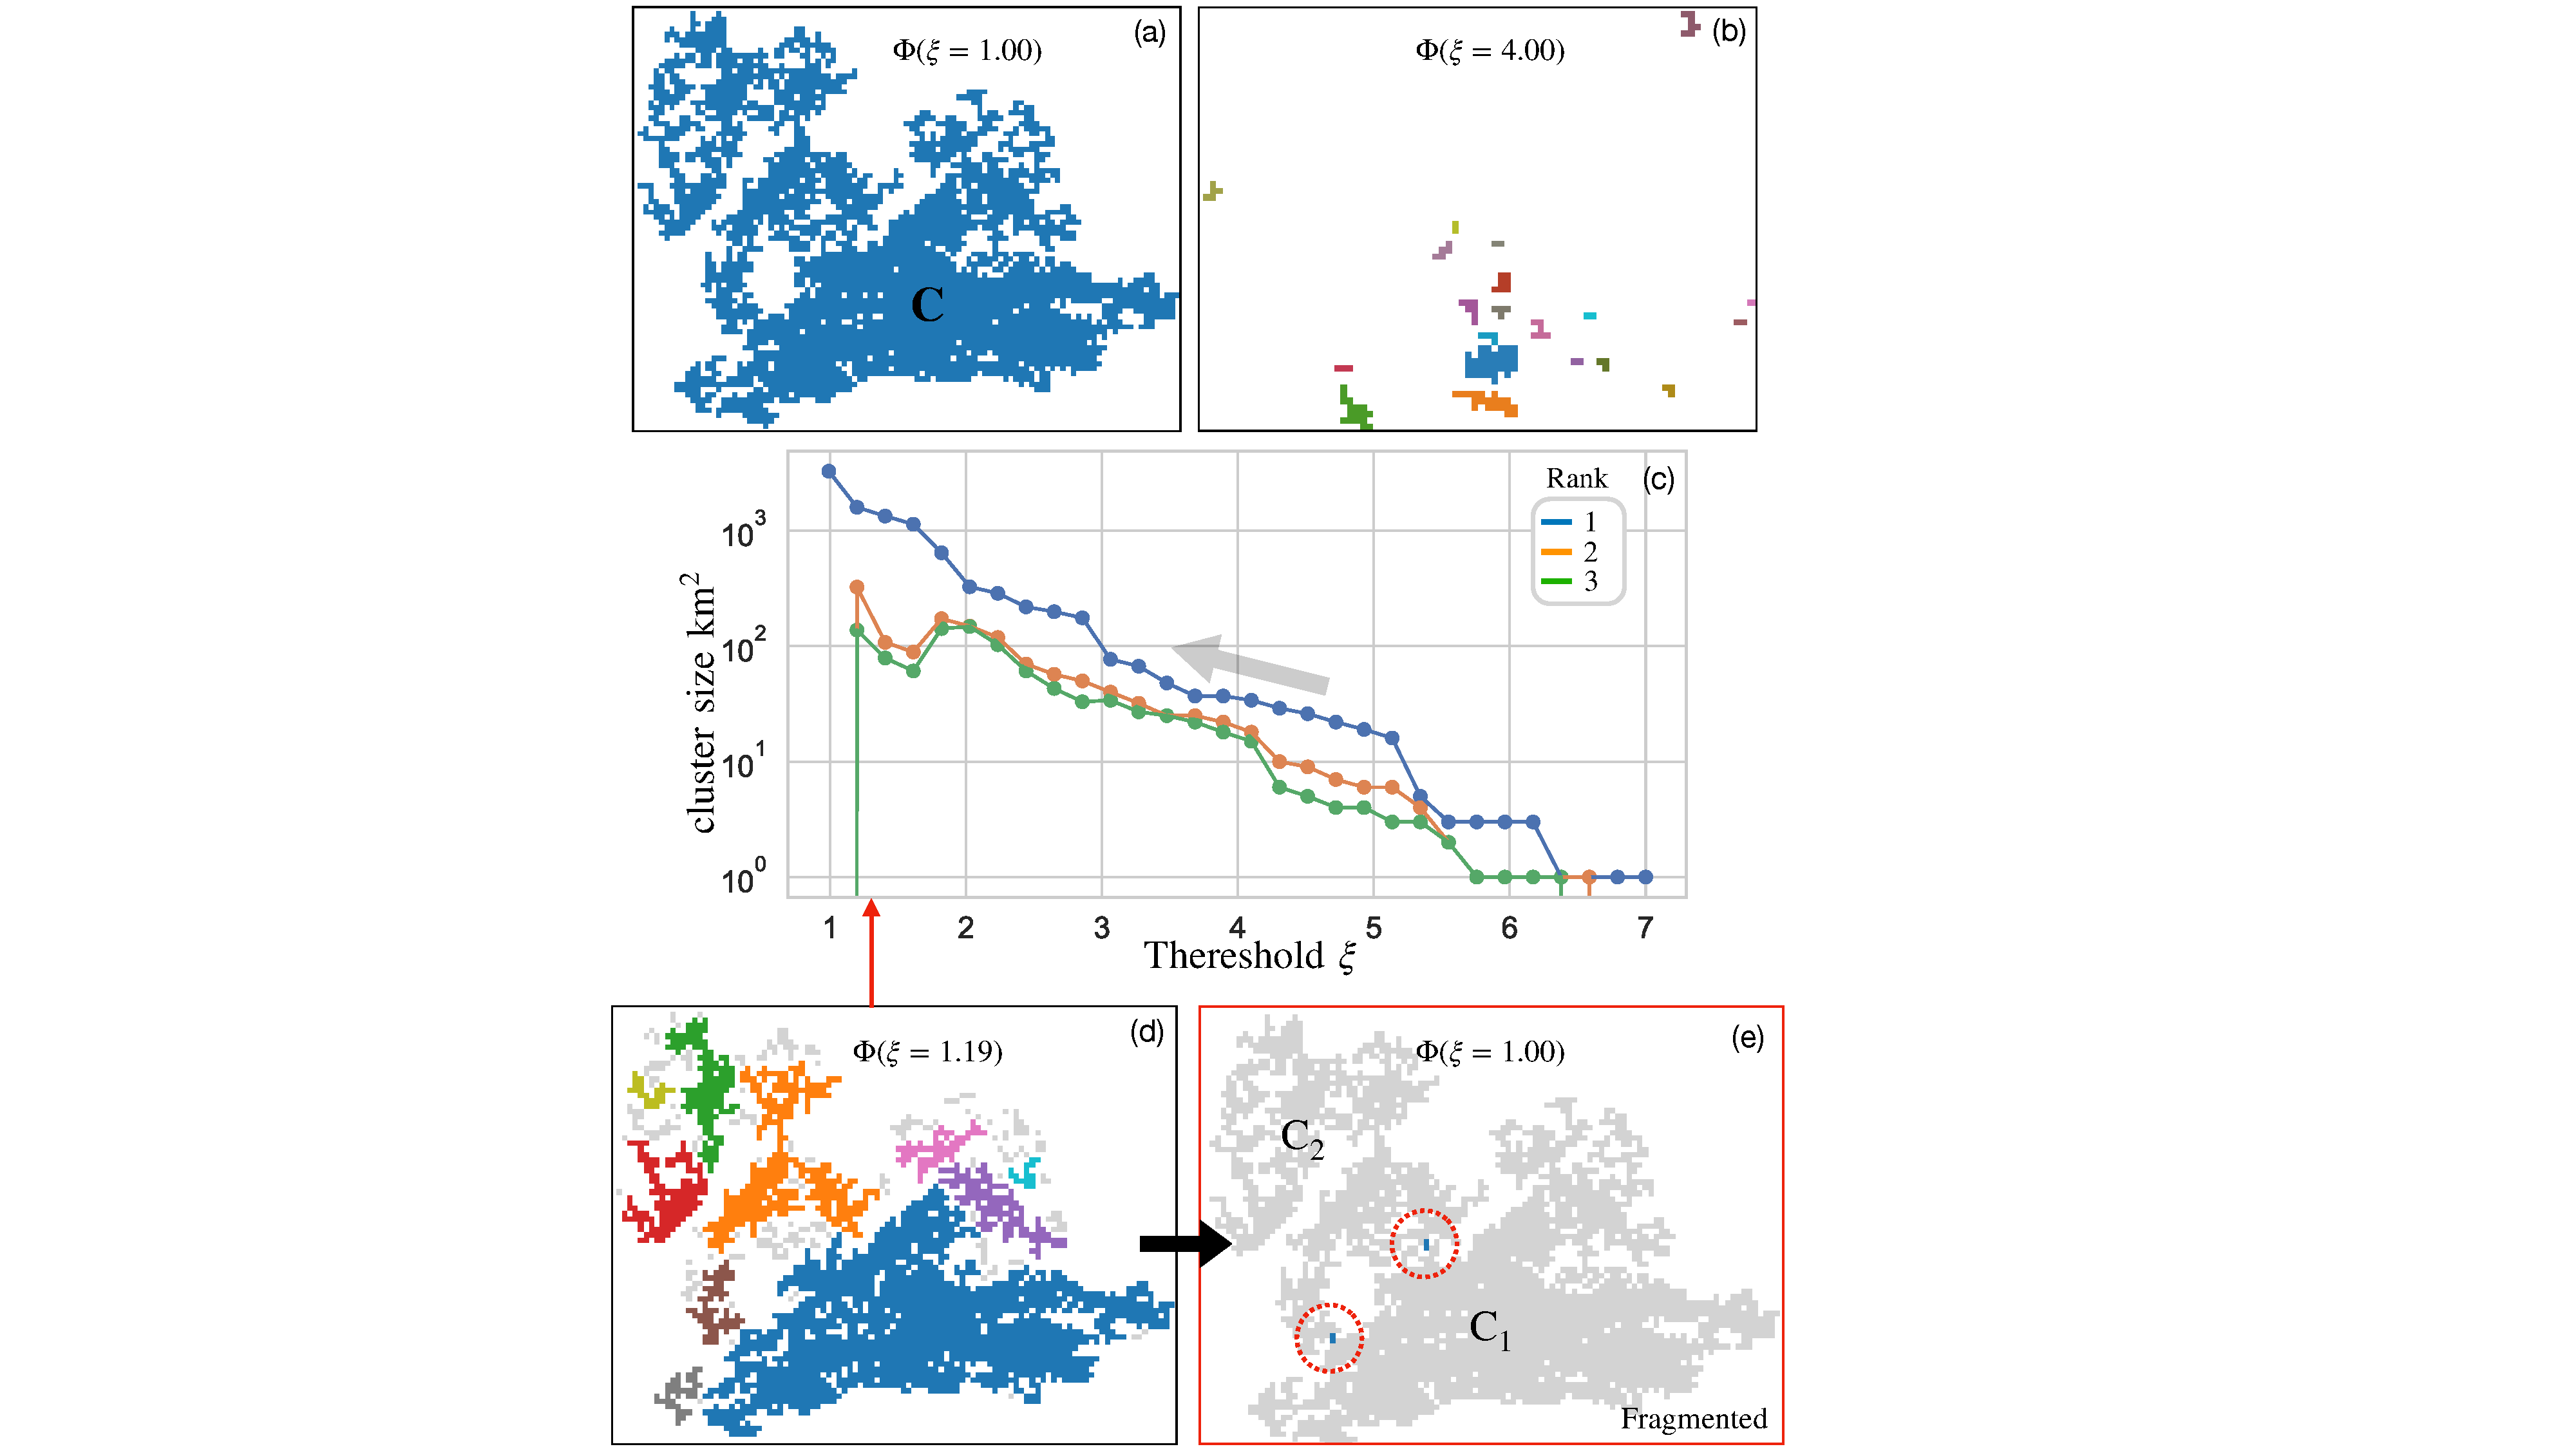
\includegraphics[scale=0.5]{chapter7/figures/figure1-frag-method.pdf}
    \caption{A graphical illustration of the algorithm developed to fragment $R_0$-clusters. 
    (a) The largest cluster, denoted by $\mathbf{C}$, is shown inside an arbitrary domain at resolution $3\mathrm{km} \times 3 \mathrm{km}$ and infectiviy $\beta^*=450$ for the model $\phi_1$-ga.
    Applying the threshold function $\Phi$ at $\xi=1$ recovers the $\mathbf{C}$ exactly, because all patches are above the threshold $R_0=1$.
    (b) Applying the threshold function $\Phi$ at $\xi=4$ yields a low-density map with sparsely distributed clusters, as few patches surpass $R_0\geq 4$. 
    (c) The top three largest clusters, by area $\mathrm{km^2}$, are shown as a function of $\xi$.
    (d) At specific values of $\xi$, some sub-clusters join to form larger clusters\textemdash here, the blue and orange clusters proceed to join at $\xi = 1.15$.
    (e) Connecting patches are identified when large discontinuities arise when back-stepping $\xi \rightarrow \xi -\delta \xi$, shown here by the blue pixels; removing these patches fragment the cluster $\mathbf{C}$ in $\mathbf{C_1}$ and $\mathbf{C_2}$. 
    }
    \label{fig:R0-threshold-function}
\end{figure}

When $\mathbf{C_1}$ and $\mathbf{C_2}$ abruptly merge and form the basis of $\mathbf{C}$, a large discontinuous jump in cluster size is detected. 
All spatial locations $(i,j)$ which bridge the gap between $\mathbf{C_1}$ and $\mathbf{C_2}$ are then identified and removed by taking $R_0$ below the threshold.
Figure \ref{fig:R0-threshold-function}(e) shows two singular patches in blue (and highlighted in red) that if taken below $R_0=1$ would fragment $\mathbf{C}$ into two sub-clusters $\mathbf{C_1}$ and $\mathbf{C_2}$.
Successive steps through $\xi$ continue until $\xi=1$.
For each discontinuity event, connecting patches are detected and removed from the system,
thus preventing $\mathbf{C_1}$ and $\mathbf{C_2}$ from merging over $\xi \in [1, R_{max}]$.
In this manor, the target-cluster $\mathbf{C}$ is fragmented into two disconnected sub-clusters. 
As we can see, connectedness within the domain can depend on a small number of patches.


% Figure \ref{fig:R0-threshold-function}(c) shows the top three largest clusters as a function of the threshold parameter $\xi$.
% As $\xi$ increases the target cluster $\mathbf{C}$ becomes progressively smaller, as fewer and fewer $R_0$ values exceed $\xi$.
% Interestingly, around specific threshold parameters (i.e. back-stepping through $\xi \rightarrow \xi - \delta \xi$), a handful of patches that
% Applying the threshold function to $\mathbf{C}$ and moving in small discrete steps backward from $\xi = R_{max}$ to $\xi=1$ will create a set of binary maps from lower to higher pixel density,
% graphically illustrated by \textcolor{red}{Figure X}(c).
% \textcolor{red}{Explain behaviour in Figure X(c)}.

\subsection{Iterative cluster fragmentation}

%  the next cluster target will be either $\mathbf{C_1}$ or $\mathbf{C_2}$, whichever has the largest number of Ash trees. 
% Iterating this $N$ times will yield $N+1$ disconnected cluster fragments.

Each $R_0$-cluster can be iteratively fragmented $N$ times to produce a set of disconnected sub-clusters, 
where, on average, each fragmentation iteration produces $N+1$ sub-divided clusters.
Figure \ref{fig:iterative-fragmentations} demonstrates the iterative process for the example cluster $\mathbf{C}$ from Figure \ref{fig:R0-threshold-function}(a).
During first iteration the target cluster $\mathbf{C}$ is fragmented into $\mathbf{C_1}$ and $\mathbf{C_2}$, shown respectively in Figure \ref{fig:iterative-fragmentations}(a) as orange and blue.
After each iteration, sub-clusters are ranked according to the area they cover, the next iteration proceeds by targeting the largest sub-cluster;
this is illustrated in Figure \ref{fig:iterative-fragmentations}(b) when $\mathbf{C_1}$ is targeted during the next iteration at $N=2$; the process is then repeated $N=10$ times to produce $11$ disconnected fragments in Figure \ref{fig:iterative-fragmentations}(c).

\begin{figure}
    \centering
    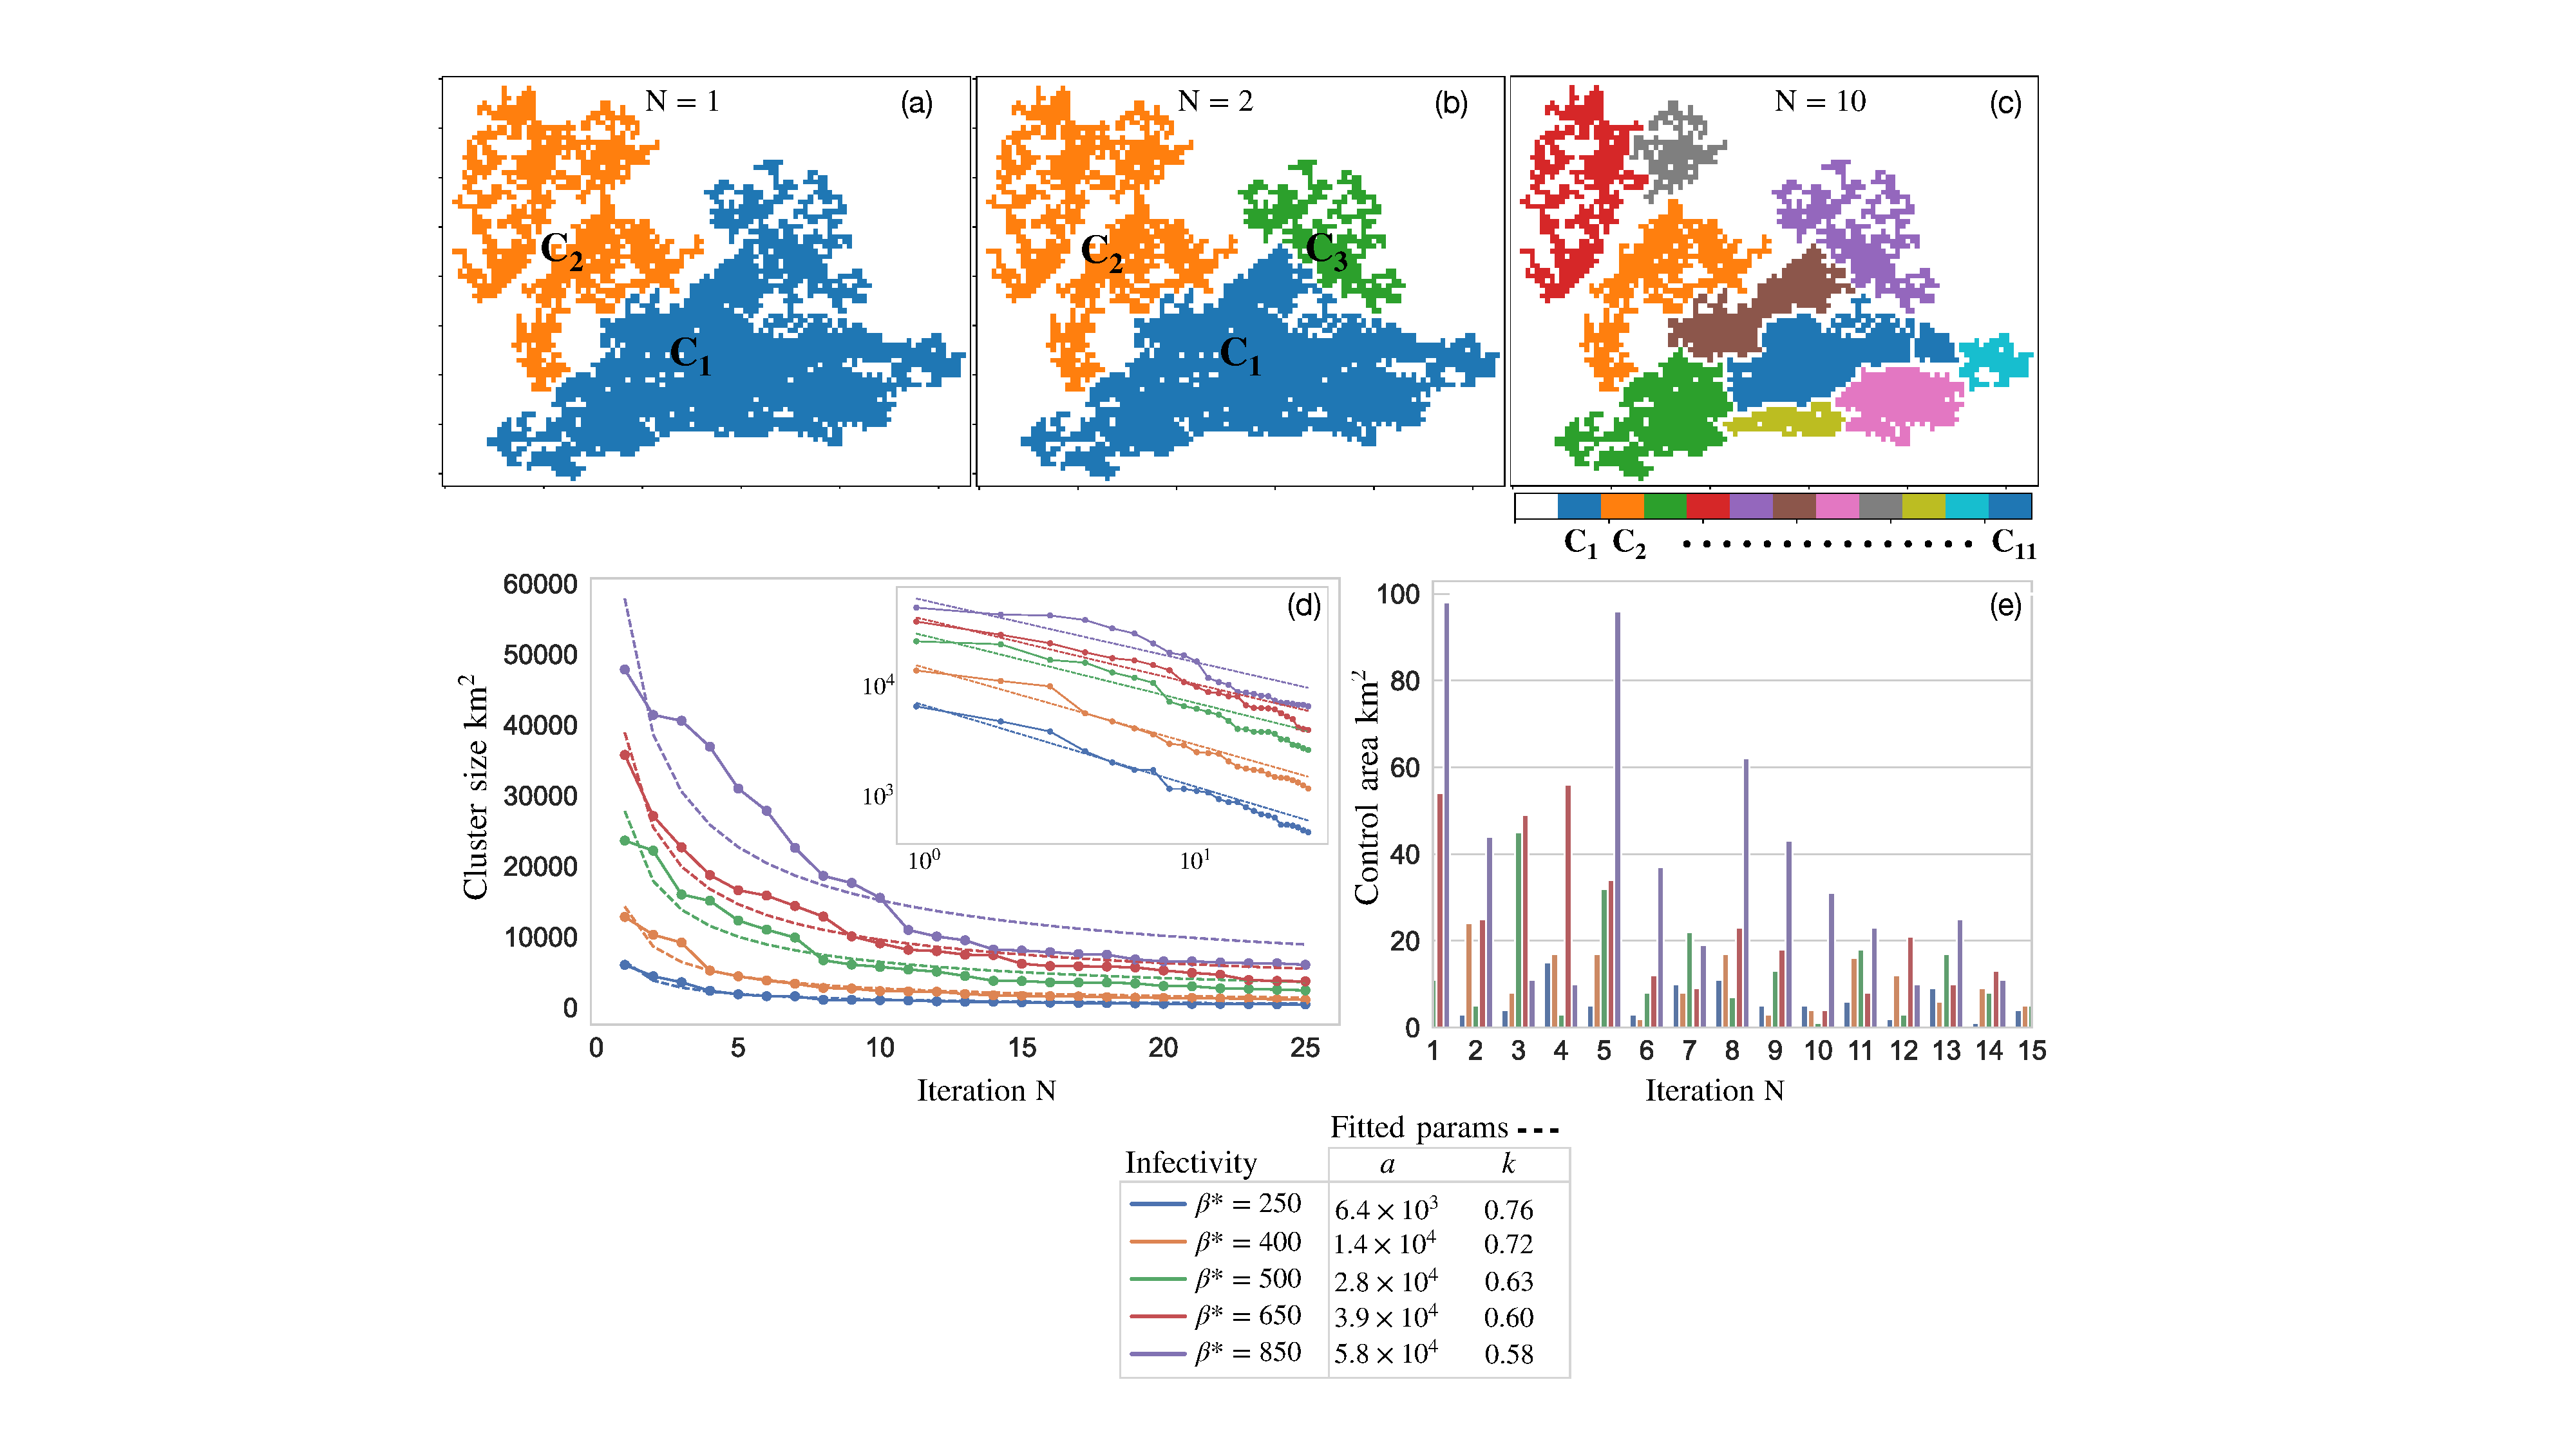
\includegraphics[scale=0.41]{chapter7/figures/figure2-Iiterative-frag.pdf}
    \caption{The fragmentation algorithm shown as an iterative process. 
    (a) The example cluster ($\mathbf{C}$) is fragmented into two sub-clusters ($\mathbf{C_1}$ and $\mathbf{C_2}$) during the first iteration of the algorithm.
    (b) During the next iteration, the largest sub-cluster $\mathbf{C_1}$ is targeted to produce an additional cluster fragment, denoted here by $\mathbf{C_3}$ in green.
    (c) The process is iteratively repeated $N=10$ times to produce $11$ sub-dived clusters.
    (d) The sub-cluster size reductions are plotted for $25$ iterations of the algorithm over a range of infectiviy parameters;  
    approximately, size-reductions follow an inverse power law, as indicated by the corresponding fitted dashed lines.
    Lower infectivity parameters correlate to a efficient fragmentation in contrast to higher $\beta^*$ values\textemdash suggested by the logarithmic inset plot.
    (e) The area of connecting patches, or `control area', is plotted against the iteration\textemdash truncated to $15$. 
    Generally, the number of connecting patches increases with infectivity and decrease with iteration.}
    \label{fig:iterative-fragmentations}
\end{figure}

Figure \ref{fig:iterative-fragmentations}(d) shows the sub-cluster size reductions for $N=25$ iterations and a number of different infectivity parameters.
For all infectivity parameters considered, the largest sub-cluster continually decreased iterations of fragmentation and size reductions occurred more rapidly at first, and slowed down as $N\rightarrow 25$.
Sub-cluster size reductions were fitted to an inverse power law of the form $f(x) = ax^{-k}$, shown by the corresponding colored dashed lines in Figure \ref{fig:iterative-fragmentations}(d).
Fitted parameter values of $a$ and $k$ represent the initial cluster size and rate of decrease respectively. 
Higher invectivity parameters can be seen to fit a larger constant $a$ and smaller exponents $k$, indicated in the legend.
Therefore, the fragmentation process becomes progressively inefficient as $\beta^*$ increases,
demonstrated most clearly by comparing the gradient of the purple and blue lines in the logarithmic inset axes\footnote{
Additionally, fragmentation was tested alongside the $2^{nd}$ and $3^{rd}$ largest $R_0$-clusters (not shown); 
for each value of $\beta^*$, $a$ and $k$ compared similarly to the $2^{nd}$ and $3^{rd}$ largest ranked clusters.}.

Lastly, Figure \ref{fig:iterative-fragmentations}(e) shows the corresponding number of connecting patches, or `control area', identified over each $\beta^*$ value and iteration.
The number of removed patches tends to decrease with iteration\textemdash most likely due to the smaller areas involved\textemdash and incrase with infectivity.
For example, when $\beta^*=850$, Figure \ref{fig:iterative-fragmentations}(e) shows a control area on the order of $100\mathrm{km^2}$,
arguably, treating a spatial extent of this magnitude would be exceedingly challenging in practice.
Thus, when $\beta^*$ becomes high it is clear to see a limitation in the framework.

% Main results figure 7

\subsection{Epidemic scenario-tests}

\textcolor{red}{Outline method to scenario tests..}
\blindtext

\begin{figure}
    \centering
    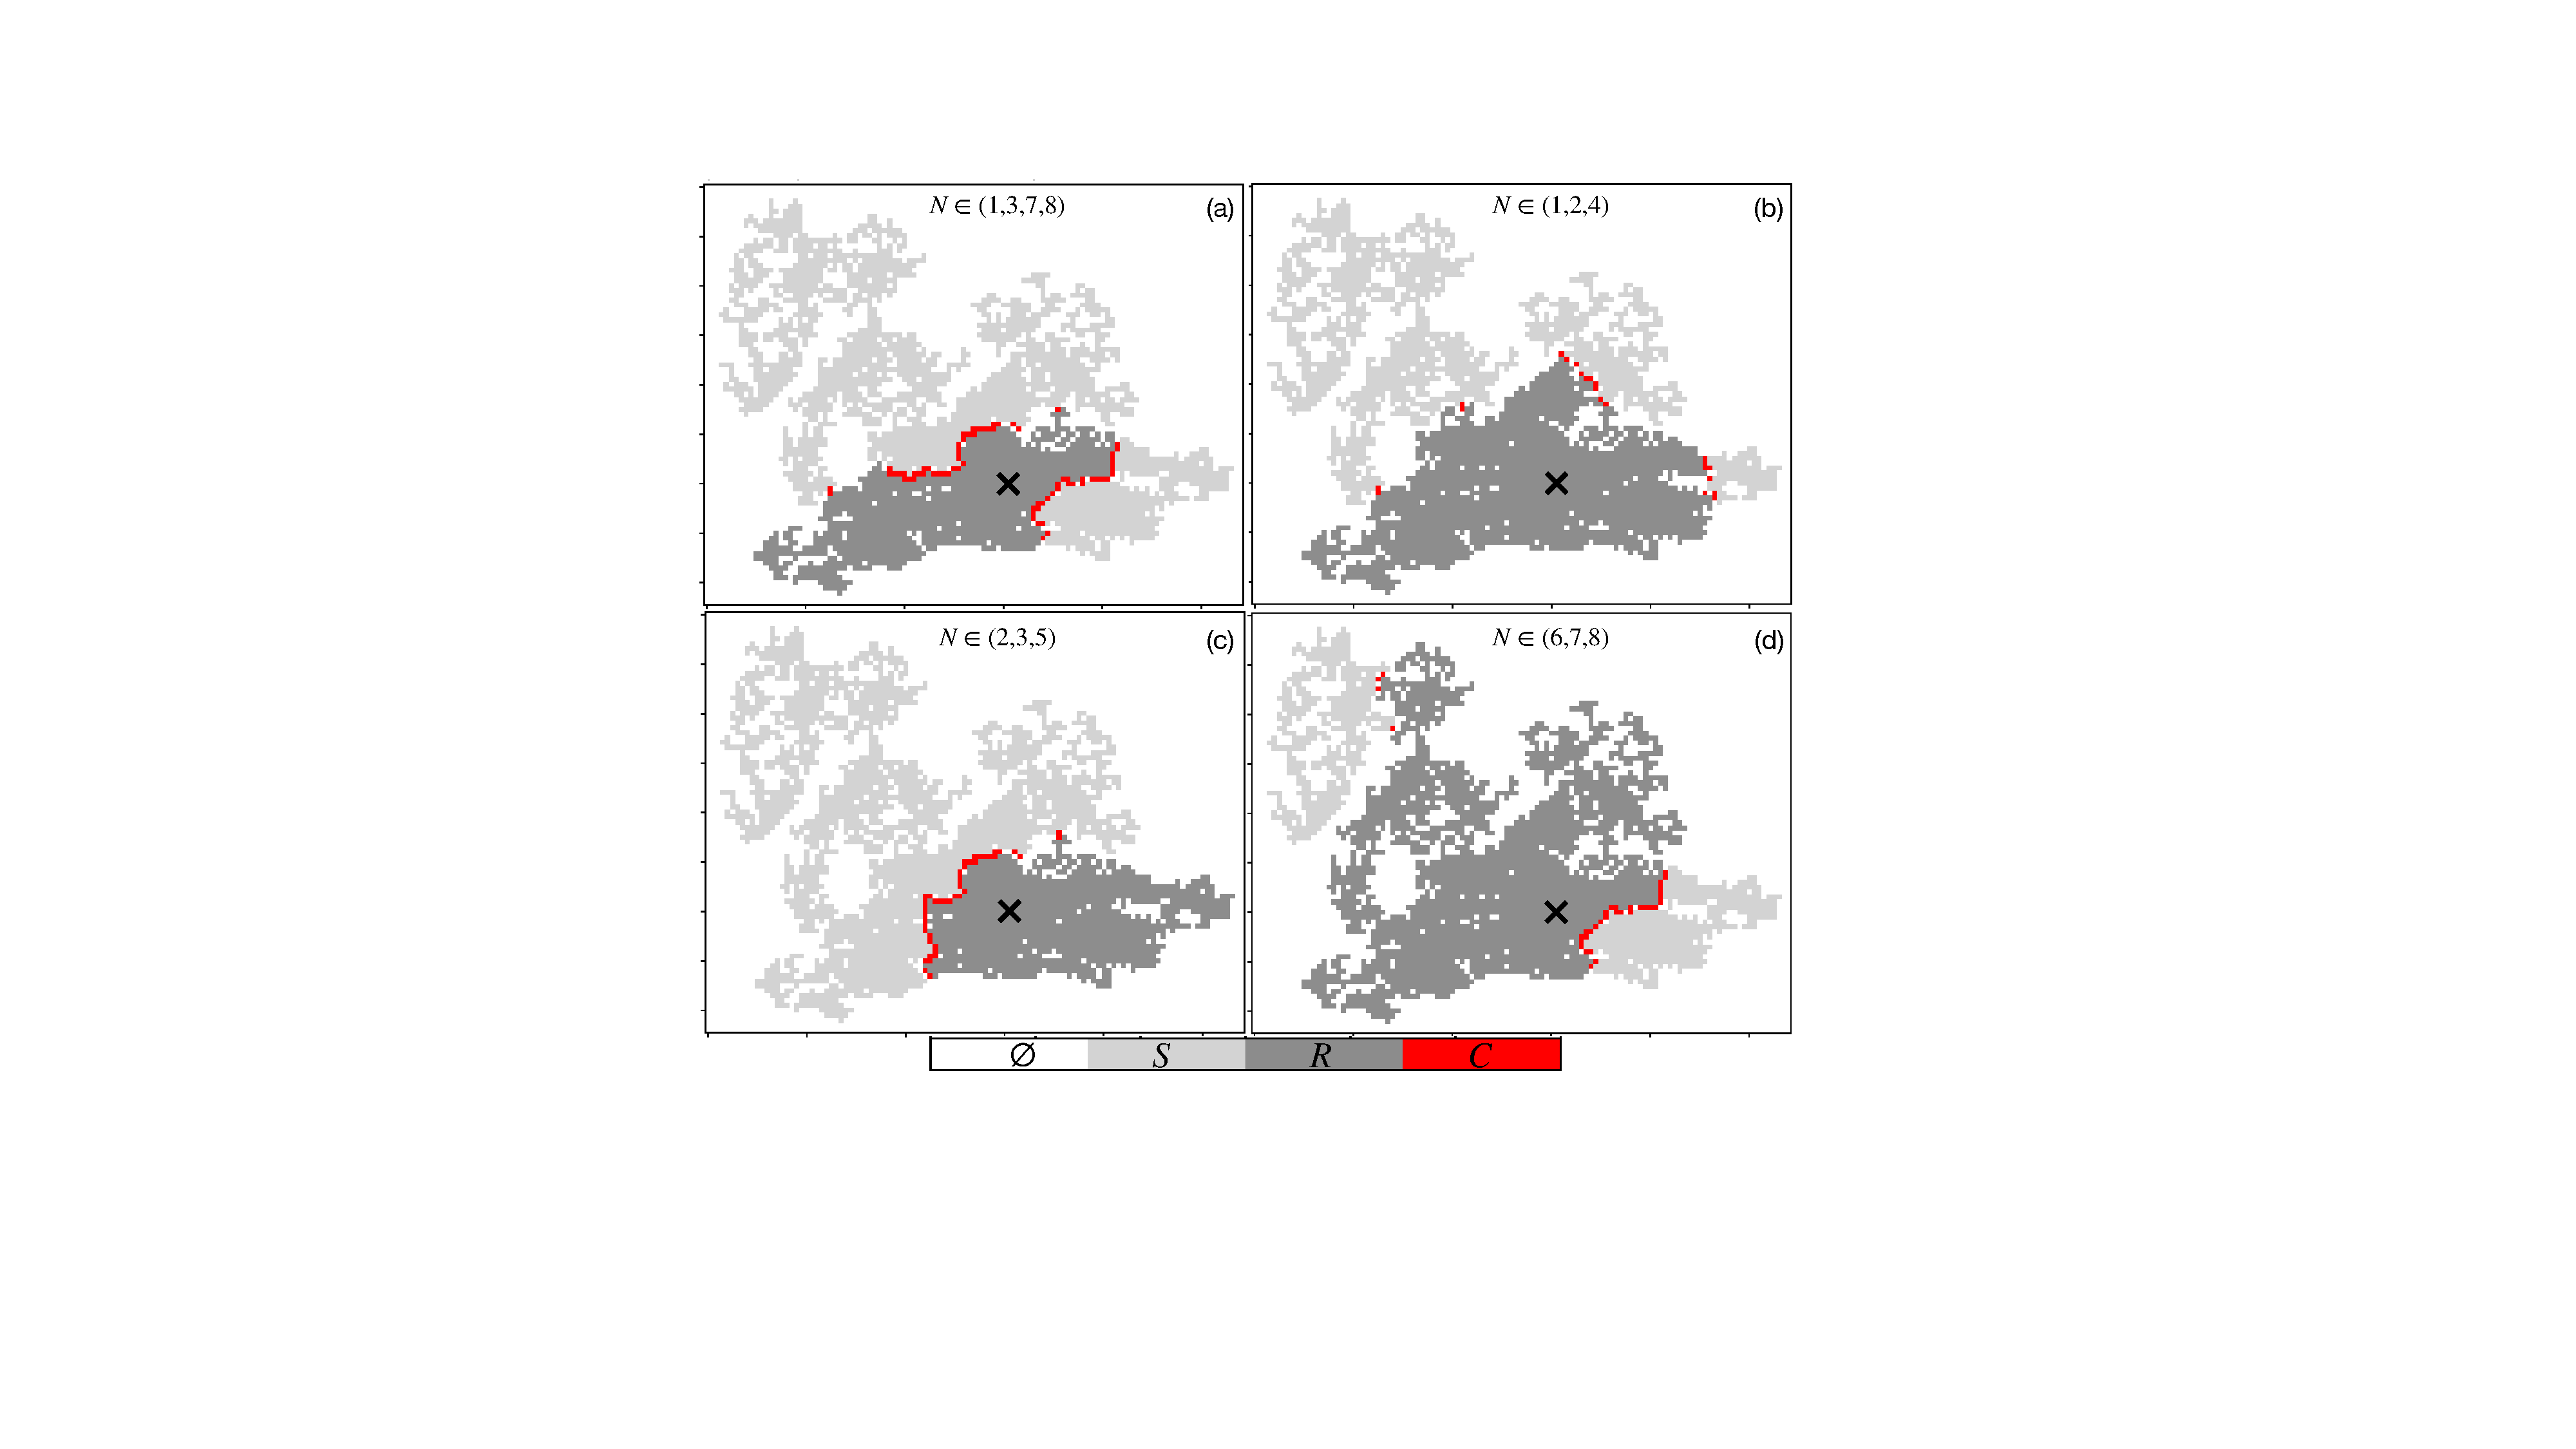
\includegraphics[scale=0.575]{chapter7/figures/figure3-scenario-test.pdf}
    \caption{For each epicenter, a variety of different control-choices are possible, based on the landscape-level host aggregation. 
    The algorithm was used to recursively fragment the target cluster $\mathbf{C}$ through $N=25$ iterations. 
    Different combinations of connecting patches can then be used to contain an epidemic in a variety of ways.
    Here, a small sample of possible control scenarios are shown for an arbitrary epicenter, depicted by the black cross.
    Red patches indicate where landscape-level control $C$ should be targeted to contain the epidemic.
    Light grey patches then remain susceptible ($S$) whilst dark grey parches are assumed at risk (or removed), denoted by $R$.
     }
    \label{fig:my_label}
\end{figure}

\blindtext

\blindtext


\subsection{Optimised landscape-level control}

\textcolor{red}{Outline method to scenario tests...}

Regional containment as a strategy of epidemic control was tested by considering outbreaks from different epicenters inside the target cluster $\mathbf{C_T}$. 
Starting from an epicenter, epidemic containment can be achieved in a variety of ways. \textcolor{red}{Figure \ref{fig:scenario-expo}} demonstrates this for a single epicenter marked by the black cross. 
The number of fragmentation iterations is varied from $N=1$ to $N=30$. 
For each step $N$, we identify which critical links, shown in red and denoted as $F$, should be felled below $\rho_c$ in order to define a confining sub-cluster around the epicenter. 
The population of saved Ash, illustrated in light grey, remains in state $S$ while all trees inside the confining sub-cluster, shown in dark grey, are assumed to transition into state $R$. 
By assessing the number of trees saved against the number of trees felled we can define a `payoff' ratio as $N_S/N_F$.

A set of epicenters were defined in $\mathbf{C_T}$ (by identifying the center of mass for each sub-cluster when $\mathbf{C_T}$ was iteratively fragmented $N=30$ times). 
From $31$ different epicenters and $30$ iterations, $930$ containment scenarios were simulated. 
For some epicenters, typically in close proximity, containment looked identical up to $N$ iterations before a different payoff ratio was registered. 
Subsequently, less than $930$ unique data-points between $N_S$ and $N_F$ were found\textemdash shown in \textcolor{red}{Figure\ref{fig:result-culling-efficiency}}.

The payoff ratios determined from the top $50$ performing containment scenarios were then ranked and plotted, 
shown in \textcolor{red}{Figure} \ref{fig:result-culling-efficiency}(a) by the blue line overlaid with a coloured scatter plot. 
For the purposes of our model, the payoff efficiency is shown alongside the corresponding number of felled trees in dashed grey. 
Payoff efficiencies begin to level off around $\mathrm{10^3}$ involving around $\mathrm{10^4}$ felled trees. 
In reality, this would be a challenge to accomplish in a reasonable time-frame. 
\textcolor{red}{Figure}\ref{fig:result-culling-efficiency}(b) shows a scatter plot of all the data, $N_S$ and $N_F$ are plotted with color corresponding to the payoff. 
The efficiency ranged over multiple orders of magnitude up to a maximum efficiency of $\mathrm{10^6}$. 
The top left quadrant of \textcolor{red}{Figure} \ref{fig:result-culling-efficiency}(b) represents viable scenarios where containment felling could be pragmatically implemented by policy makers with the greatest efficiency.

A small number of exceedingly high payoff results were found. 
In \textcolor{red}{Figure}\ref{fig:result-culling-efficiency}(c), the top three ranking payoff scenarios are illustrated on the same map and reinforces the intuitive notion that epicenters around edge positions can be most efficiently contained. 
The zoomed inset highlights just $\mathrm{2\times 1km^2}$ Ash patches located at a single point of contact for the top ranked sub-cluster. 
Critical links for the best performing scenarios were all found in lower-density regions within the $R_0$-cluster and were easily fragmented with a low number of felled trees. 
This highlights the possibility that fragmentation is most easily achieved with tree felling through critically linking regions and
demonstrates how regional variation in host density can be exploited for efficient control. 

\section{Case-study: patch-level density-reductions \\ (unfinished)}
\label{sec:cast-study-jump-patches}
\textcolor{red}{\blindtext}

\section{Chapter summary}

The article published by \cite{time-varying-infectivity} indicates the possibility of \textit{preferentially} controlling an area based on the final-sized epidemic. 
It goes without saying that areas of land that have the largest final sized epidemic are likely the most density populated. 
However, we outline the possibility it might be more beneficial to preferentially control an area based on its spatial location and how it couples to to neighbouring areas.

% genetic tolerance is currently the only viable strategy of control\cite{kosawang2018fungal}

% Crucially, future work will involve integrating LDD mechanisms into the model in order to understand the relative importance long vs local distance dispersal. We may speculate about the relative importance looking at figure x, whereby the maximum distance spread in season due to local-scale spread is xm/year, in stark contrast from the observed spread of 40-60km/yr.

% We cannot overstate the importance of LDD, and it is hard to say the degree to which targeting the local dispersal mechanism alone will inhibit the spread. We will revisit this question in future work, however, we contend that preferentially targeting diseased trees based on spatial location.....could help control epidemics with greater efficacy. 

% We may speculate how our result could aid the effort of choosing where to re-plant ash stands genetically engineered to be less susceptible; if re-planting efforts were undertaken in certain location.... <- speculative

% We may speculate about how persistent ash dieback would be, even if a large-scale control effort was undertaken

% There is evidence to suggest regional variation in mortality due to ash dieback \cite{stocks2017first}, this could be incorporated into the model...

% Our results support the call for more research to be undertaken into multi-scale dispersal, 

% Recently, it has been suggested that the dispersal-kernel of wind-borne pathogens might follow a scaling law \cite{https://doi.org/10.1111/jbi.13642}. The significance of such a finding would allow us to analyse the $R_0$-maps over much more flexible spatial scales. % Explain.

% This sentence is wrong, the cited paper makes an argument for the spatially-scaling up of dispersal kernels, which happens to still be useful paper to cite, re-phrase and re-frame accordingly.

% see \cite{ash-dieback-costs}, and the references therein (methodology excel spread sheet S1), for mortality references the latest findings suggest a mean mortality rate of 95%.
